\documentclass[../rapport_MVEX01-11-05]{subfiles}
\begin{document}

\section{Klassificering av gester med hjälp av \knn}
Den största andelen korrekt klassificerade gester vi lyckades uppnå var 91,5\%.
Denna andel uppnåddes då samtliga gester var inkluderade. Antalet aktiverade
egenskaper var 10 och antalet närmsta grannar i \knn-metoden var 7 --- denna
konfiguration nåddes genom optimering i $k$-led och av mängden inkluderade
egenskaper. Egenskaperna som
användes är listade i tabell~\ref{tab:bestfeats}.
Figur~\ref{fig:knn-optimering} visar mer exakt hur andelen korrekta
klassficeringar beror på antalet aktiverade egenskaper och värdet på $k$.

\begin{figure}[tbp]
  \centering
  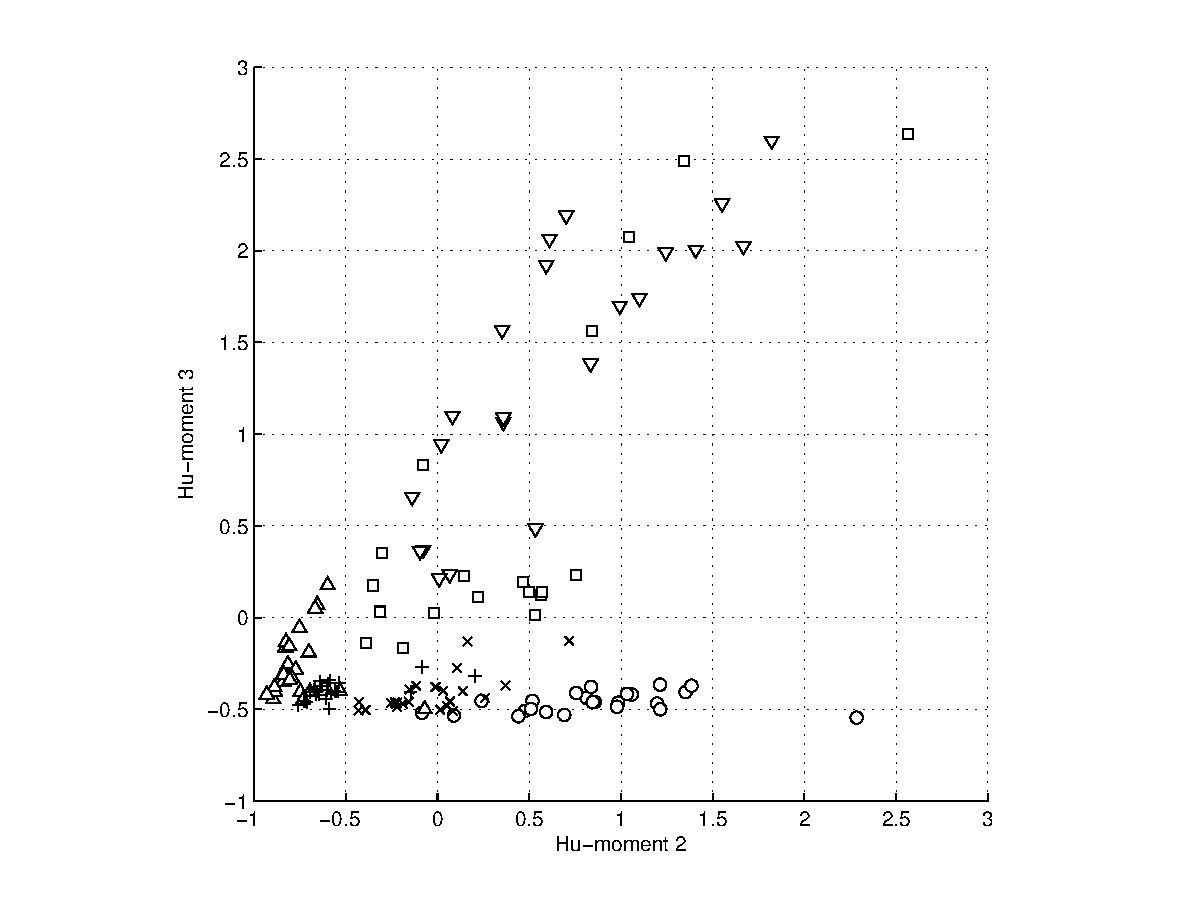
\includegraphics[width=\textwidth,trim=2cm 0.5cm 2cm 0,clip=true]{bilder/feats-10+11}
  \caption{Träningsmängden för ett urval av gester plottat mot de två starkaste
  egenskaperna. \notes{Tydliggör att punkterna är olika}}
  \label{fig:feats1011}
\end{figure}

\begin{figure}[tbp]
    \begin{center}
        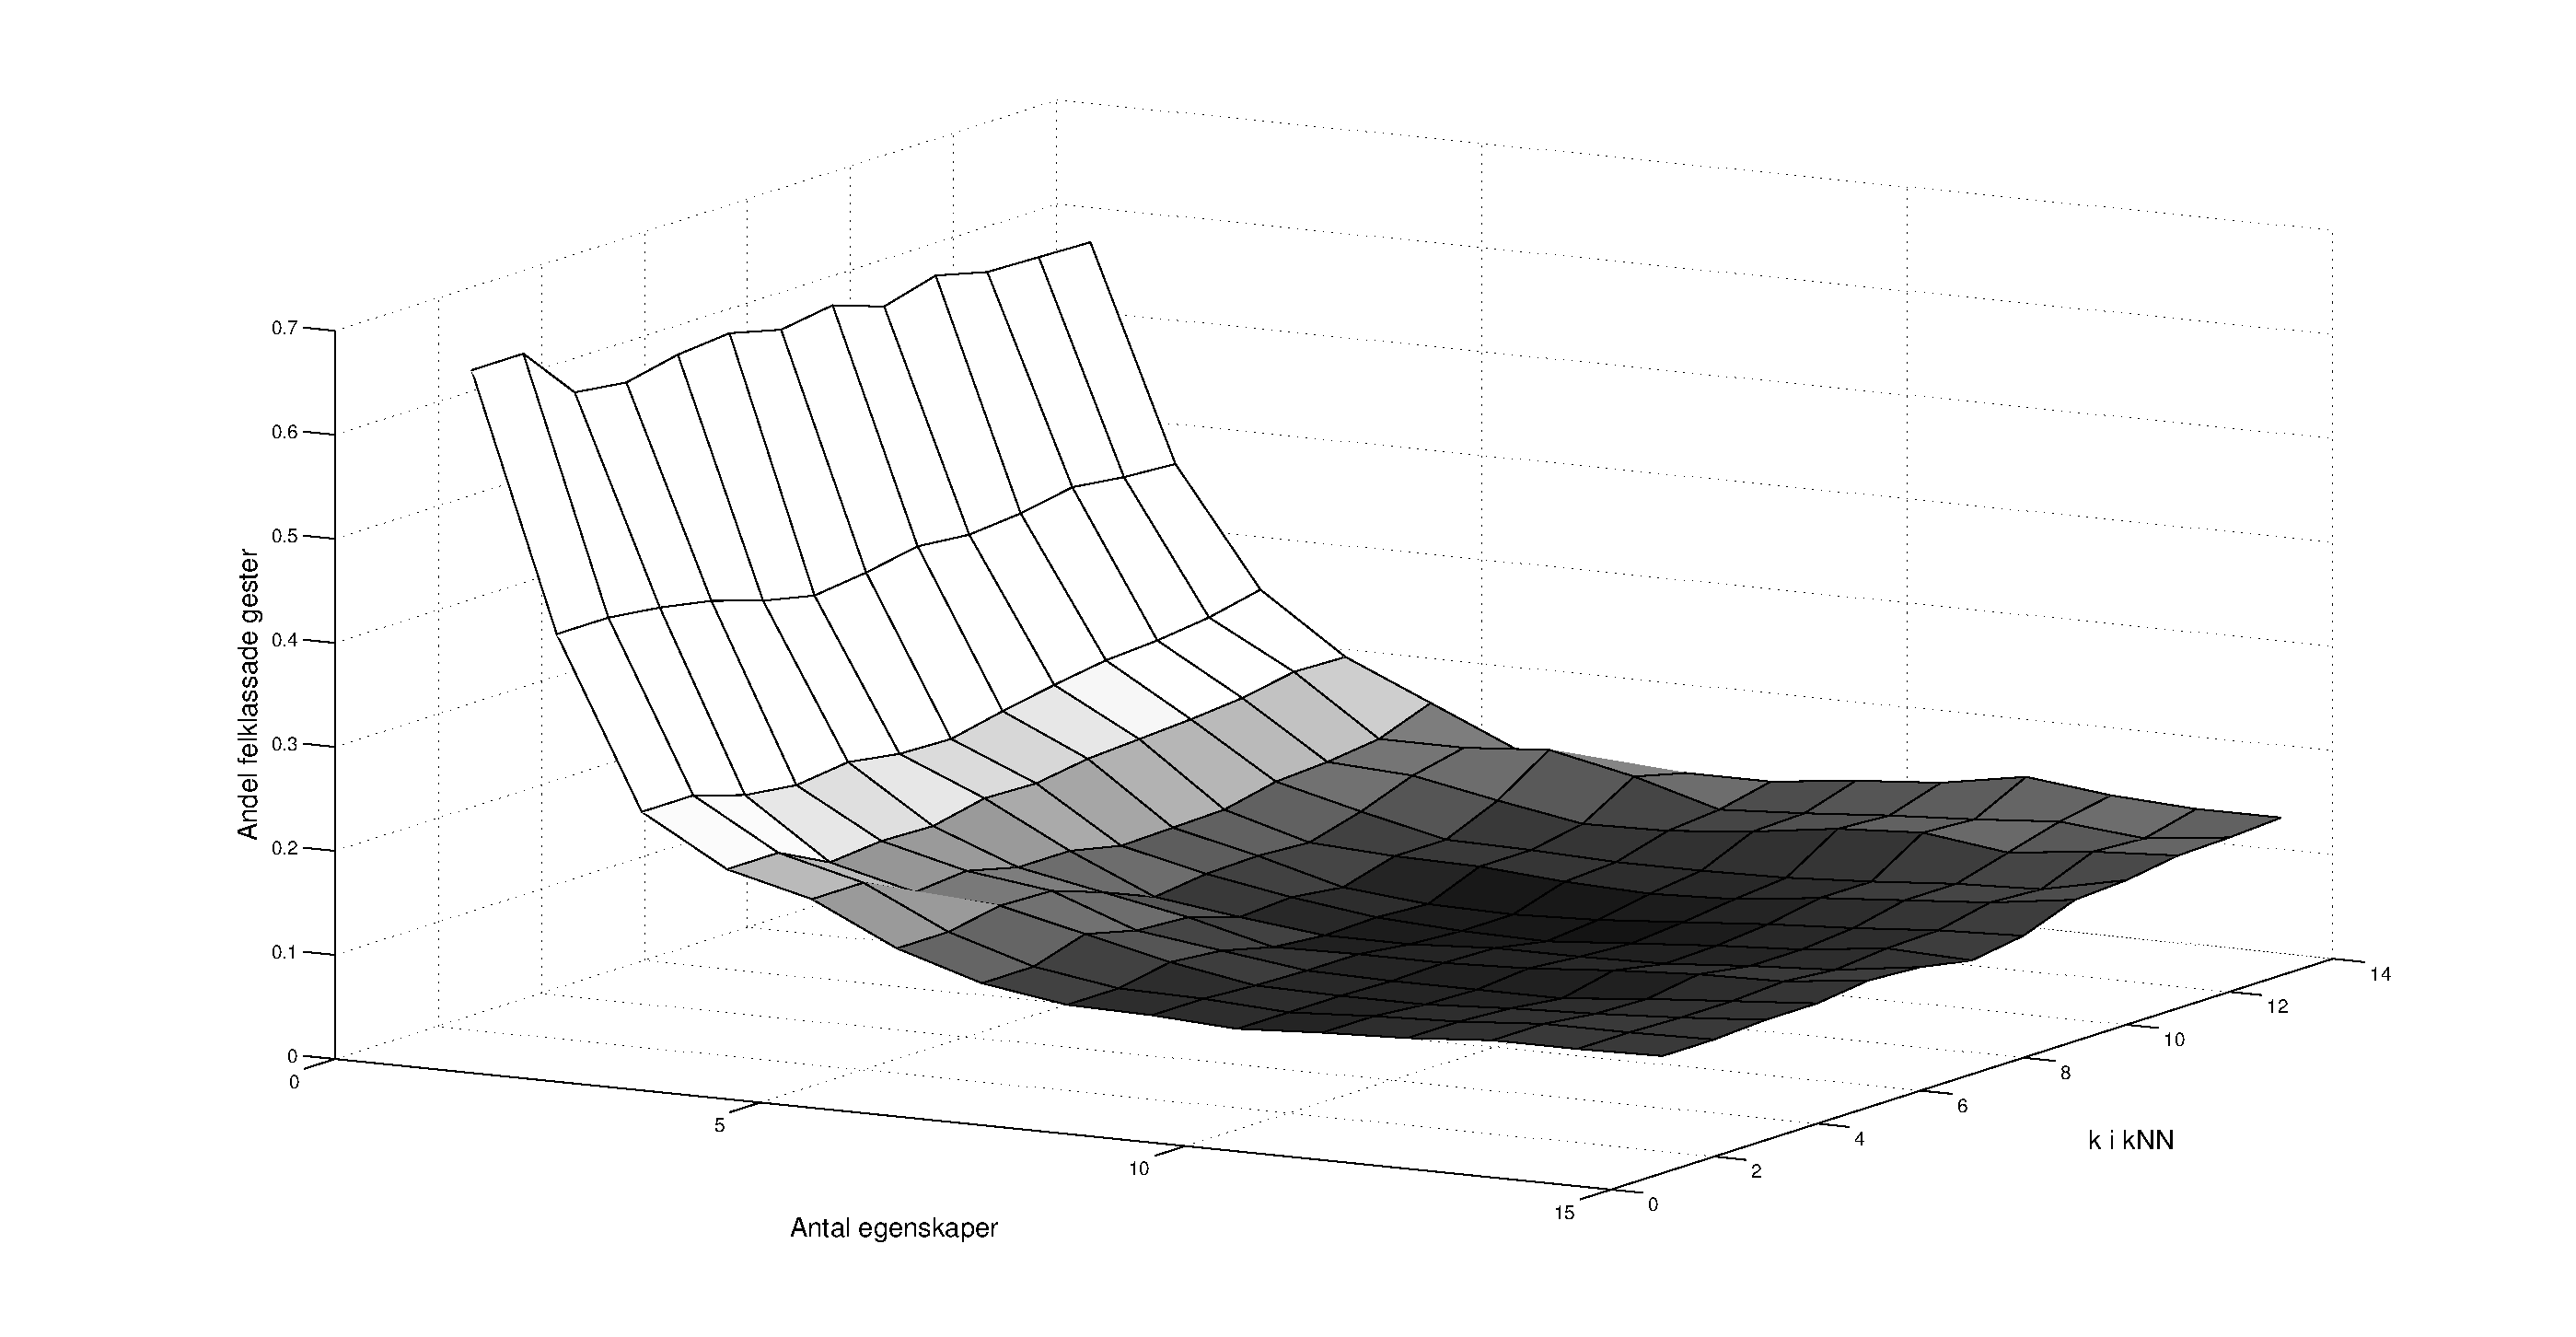
\includegraphics[trim=2cm 2cm 2cm 1.8cm,width=\columnwidth,clip=true]{bilder/knn_optimering.pdf}
    \end{center}
    \caption{Optimering av \knn-metoden med avseende på inkluderade egenskaper
och värder på $k$ ger ett tydligt minimum då $k=7$ och 10 egenskaper inkluderades}
    \label{fig:knn-optimering}
\end{figure}

Det framgår tydligt att antalet aktiverade egenskaper har stor
inverkan på resultatet då man använder sig av färre än
fem. Därefter planar andelen ut för att återigen stiga då
fler än 10 egenskaper används. Andelen felklassificeringar
minskar också i takt med att $k$ ökar från 1 till 7, för att sedan
öka då värdet ökar från 7 till 13. Med det optimala
valet av egenskaper och $k$ presterade metoden enligt
tabell~\ref{tab:tolkningsmatris} och tabell~\ref{tab:prestanda}.

\notes{(Inkludera resultat där problemgester är borttagna?)}

\begin{table}[tbp]
	\centering
	\caption{SKRIV MIG!!!}
	\label{tab:prestanda}
	\begin{tabular}{c c c}
		\toprule 
		Försöksgest & Feltyp 1 & Feltyp 2 \\
		\midrule 
		A & & \\
		B & & \\
		C & & \\
		D & & \\
		E & & \\
		Sten & & \\
		Sax & & \\
		Påse & & \\
		Spock & & \\
		Seger & & \\
		\bottomrule 
	\end{tabular}
\end{table}

\begin{table}[tbp]
	  \centering
		\caption{Vid försök misstolkas en del gester betydligt oftare än
		andra. Notera att raderna inte adderar till 100 eftersom värdena är
		avrundade.}
		\label{tab:tolkningsmatris}
    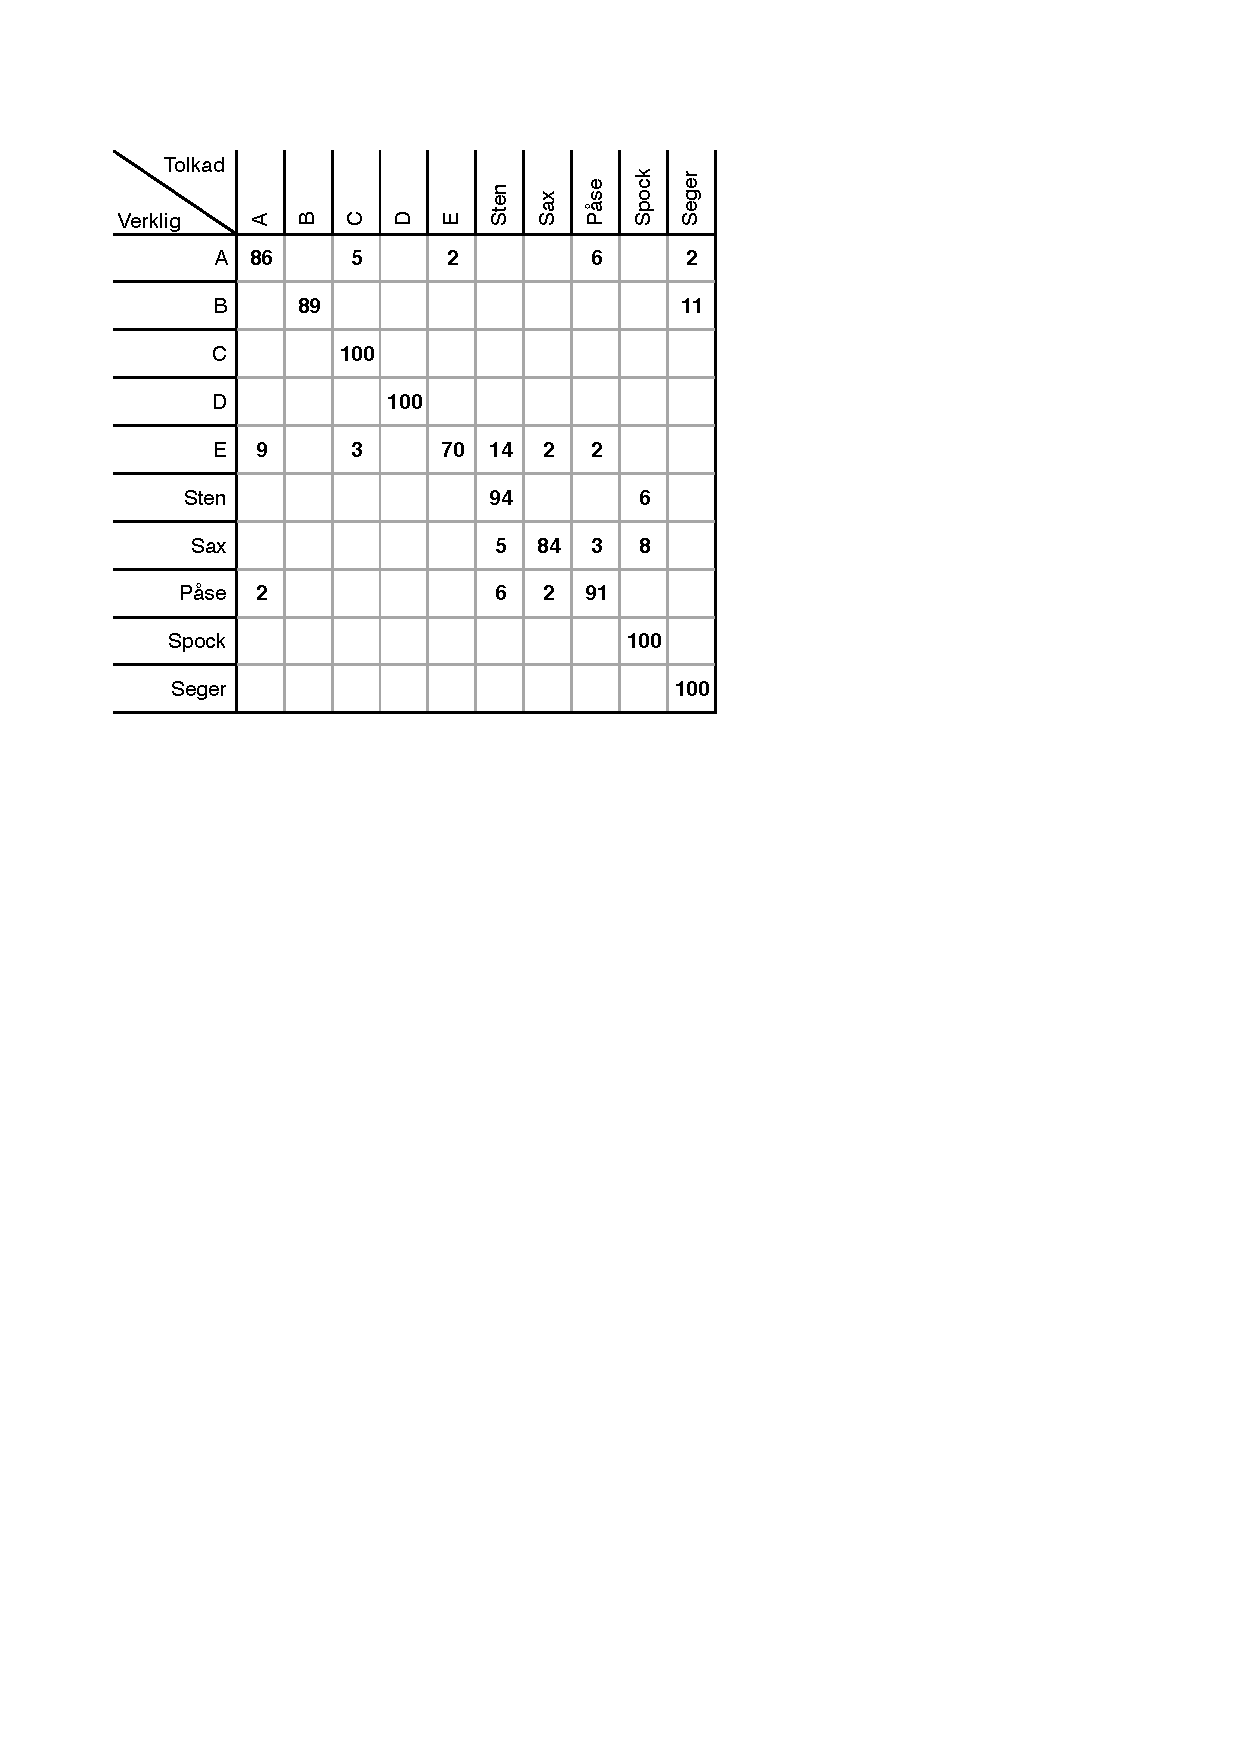
\includegraphics[trim=2cm 16cm 8cm 2.5cm,clip=true,width=8cm]{bilder/tolkningsmatris.pdf}
\end{table}

\begin{table}[tb]
	\centering
	\caption{De tio bästa egenskaperna}
	\label{tab:bestfeats}
	\begin{tabular}{ll}
		\toprule
		Ranking & Egenskap \\
		\midrule
		1 & Hu-moment 3 \\
		2 & Hu-moment 2 \\
		3 & Centroidläge, Y-led \\
		4 & Fyrkantighet \\
		5 & Soliditet \\
		6 & Excentricitet \\
		7 & Konvexitet \\
		8 & Hu-moment 1 \\
		9 & Utsträckning \\
		10 & Hu-moment 7 \\
		\bottomrule
	\end{tabular}
\end{table}

\subsection{Egenskaper}\label{sec:resultat_features}

Egenskaperna vi använt har visat sig vara mycket bra, upp till en viss gräns.
Figur~\ref{fig:knn-optimering} visar att optimering av vilka egenskaper som
inkluderas ger ett distinkt minimum redan vid tio egenskaper --- dessa tio
bästa listas i tabell~\ref{tab:bestfeats}.

\end{document}
